\documentclass[crop,class=article]{standalone}
%----------------------------Preamble-------------------------------%
\usepackage{amssymb}
\usepackage[dvipsnames]{xcolor}         % Color names.
\usepackage{tikz}                       % Drawing/graphing tools.
\usetikzlibrary{arrows.meta}            % Latex and Stealth arrows.
\DeclareMathSymbol{\minus}{\mathbin}{AMSa}{"39} % Unary minus sign.
%--------------------------Main Document----------------------------%
\begin{document}
    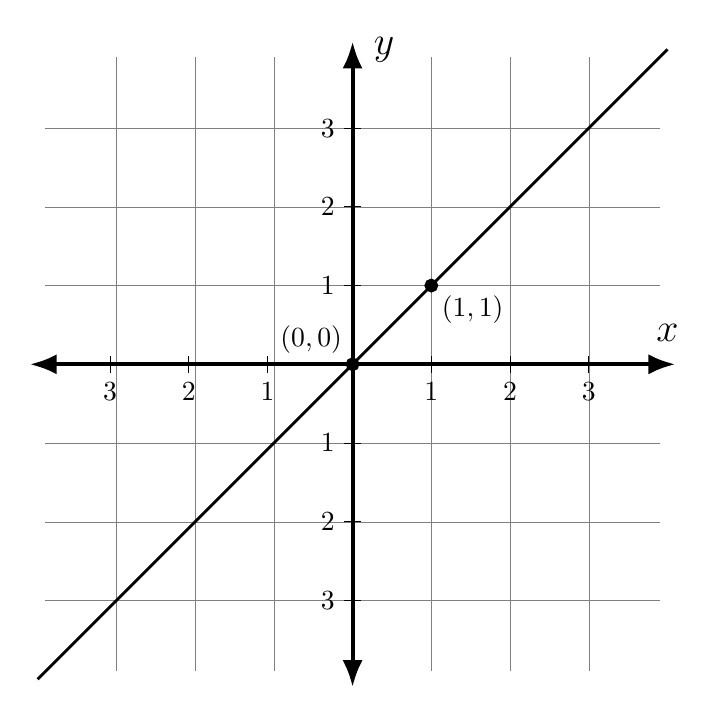
\begin{tikzpicture}[>=latex, line width=1pt]
        \draw[style=help lines] (-3.9, -3.9) grid (3.9, 3.9);
        \begin{scope}[line width=0.3pt]
            \foreach\n in {1,2,3}{%
                \draw (\n,3pt) -- (\n,-3pt) node [below] {$\n$};
                \draw (3pt,\n) -- (-3pt,\n) node [left] {$\n$};
                \draw (-\n.08,3pt) -- (-\n.08,-3pt) node [below] {$\minus\n$};
                \draw (3pt,-\n) -- (-3pt,-\n) node [left] {$\minus\n$};
            }
        \end{scope}
        \begin{scope}[line width=1.5pt, >=Latex, font=\Large]
            \draw[<->] (-4.1, 0) to (4.1, 0);
            \draw[<->] (0, -4.1) to (0, 4.1);
            \node at (4, 0.4) {$x$};
            \node at (0.4, 4) {$y$};
        \end{scope}
        \draw (-4, -4) to (4, 4);
        \draw[fill=black] (0,0) circle (0.7mm) node[above left] {$(0,0)$};
        \draw[fill=black] (1,1) circle (0.7mm) node[below right] {$(1,1)$};
    \end{tikzpicture}
\end{document}